\documentclass[pdftex,12pt,a4paper]{report}

\usepackage[pdftex]{graphicx}
%\usepackage[ansinew]{inputenc}
\usepackage{geometry}
\usepackage{bbold}
\usepackage[T1]{fontenc}
\usepackage[utf8]{inputenc}
\usepackage[english]{babel}
\usepackage{url}
\usepackage{subfigure}
\usepackage{hyperref}
\usepackage[section]{placeins}
\usepackage{listings}
\usepackage{wrapfig}
%\usepackage{titlesec}
\usepackage[Sonny]{fncychap}
\usepackage[table,xcdraw]{xcolor}
\geometry{a4paper,left=2.5cm,right=2.5cm, top=2.5cm, bottom=3cm}
\newcommand{\HRule}{\rule{\linewidth}{0.5mm}}
%\titleformat{\chapter}
 % {\normalfont\bfseries\Huge}{\thechapter.}{12pt}{}

\makeatletter
\ChTitleVar{\Large\rm\centering} % sets the style for title
\ChNameLowerCase
\renewcommand{\DOCH}{}
\makeatother

\begin{document}
\begin{titlepage}


%%LR
\sffamily

\begin{center}


% Oberer Teil der Titelseite:

\includegraphics[width=0.3\textwidth]{bilder/logo2.jpg}
\hfill

\includegraphics[width=0.4\textwidth]{bilder/logo1.jpg}  
\\[5cm]

{\Large Bioinformatics Program}\\[0.5cm]
{\Large Technical University of Munich}\\[0.5cm]
{\Large Ludwig-Maximilians-Universit\"at M\"unchen}\\[2cm]
{\Large Master's Thesis in Bioinformatics}\\[1.5cm]

% Title
\HRule \\[0.4cm]
{ \huge \bfseries Patient-specific dysregulation analysis based on gene regulatory networks in cancer}\\[0.4cm]

\HRule \\[1.5cm]

{\Large Sebastian Dötsch}\\[2.5cm]

\vfill
\end{center}
\end{titlepage}
\pagestyle{empty}

%%LR comprehensive title
\begin{titlepage}
{\sffamily


\begin{center}

\includegraphics[width=0.3\textwidth]{bilder/logo2.jpg}
\hfill

\includegraphics[width=0.4\textwidth]{bilder/logo1.jpg}  
\\[3cm]  

{\Large Bioinformatics Program}\\[0.5cm]
{\Large Technical University of Munich}\\[0.5cm]
{\Large Ludwig-Maximilians-Universit\"at M\"unchen}\\[2cm]
{\Large Master's Thesis in Bioinformatics}\\[2cm]
{\textbf{\LARGE Patient-specific dysregulation analysis based on gene regulatory networks in cancer}}\\[2cm]
{\textbf{\LARGE Patientenspezifische Dysregulationsanalyse bei Krebs basierend auf genregulatorischen Netzwerken}}\\[3cm]

\end{center}
\begin{center}\Large
  \begin{tabular}{ll}
    Author:& Sebastian Dötsch\\
    Supervisor: &  Dr. Markus List Chair of Experimental \\
    & Bioinformatics,\\
    & TUM School of Life Sciences Technische Universität\\
    & München \\
    & Dr. Josch Pauling LipiTUM, Chair of Experimental \\
    & Bioinformatics, \\
    & TUM School of Life Sciences Technische Universität \\
    & München\\
    Advisor:        &  Alexander Dietrich, Technische Universität München\\
    Submitted:     &  15.09.2023
  \end{tabular}
\end{center}

}% end title page

\end{titlepage}

\newpage
\phantom{oben}
\vfill
\begin{center}
\large\textbf{Declaration of Originality}\normalsize\\
\vspace{0.5cm}
I confirm that this master's thesis is my own work and I have documented all sources and material used.\\
\vspace{1.5cm}
\begin{tabular}{lp{2em}l}
 \hspace{3cm}   && \hspace{3cm} \\\cline{1-1}\cline{3-3}
 Ort, Datum     && Unterschrift
\end{tabular}
\end{center}
\vfill

\tableofcontents

\chapter*{Abstract}

\chapter{Introduction}

\section{Epigenetics}
Epigenetics, an emerging field in molecular biology, gives insights into heritable gene regulation. It involves dynamic changes in DNA, chromatin, and noncoding RNAs. DNA methylation the field this work focuses on will be discussed in more detail in the further course. Simultaneously, histone tail modifications, including acetylation and methylation, control chromatin structure and influence gene accessibility\cite{epigenetics_histone}. Noncoding RNAs such as microRNAs fine-tune gene expression post-transcriptionally. Epigenetics offers insights into development, disease, and therapeutic opportunities\cite{epigenetics_nonRNA}. This dynamic interplay between genetic and epigenetic mechanisms opens new approaches for our understanding of biological complexity and is therefore investigated.
\subsection{DNA Methylation}
DNA methylation, an important epigenetic modification, involves the addition of methyl groups to cytosine or adenine bases in DNA molecules. It typically occurs on the first mentioned by addition of the methyl group to the carbon-5 atom of cytosin. This reaction is catalyzed by the three DNA methyltranferases DNMT3A, DNMT3B and DNMT1. DNMT3A and DNMT3B are essential for de novo methylation, for example during embryogenesis and germ cell development \cite{methylation_dnmtsAB}. DNMT1 on the other hand is responsible for maintaining methylation patterns and does this by catalyzing the addition of methyl groups to cytosine nucleotides \cite{methylation_dnmts1}. Therefore this chemical alteration is involved in cellular development and maintenance of genome integrity. It regulates gene expression by inhibiting the binding of transcription factors (TFs) to DNA or recruiting repressor genes \cite{gene_regulation}. It additionally silences a large number of parasitic transposable, retroviral, repeat elements, which the mammalian genome gathered over time \cite{MethRole}.

DNA methylation occurs very frequently at CpG sites (CpGs), 70\% to 80\% of CpG cytosines are methylated in mammals\cite{methylation_cpg}.
CpGs are regions in the DNA where a cytosine nucleotide is followed by a guanine nucleotide, if they occur with a atypically high frequency in a sequence it is called a CpG island\cite{cpgislandguide}.
These sites hold a central role in gene expression regulation, acting as epigenetic switches when located in promoter regions of genes\cite{cpgisland}. 
Beta values, a critical metric in DNA methylation studies, quantify the degree of DNA methylation at CpG sites. By taking the methylated (\emph{M}>0) and unmethylated (\emph{U}>0) signal intensities, measured by the Illumina 450k array the beta value \emph{b}=\emph{M}/(\emph{M}+\emph{U}+\emph{a}) is calculated. To stabilize beta values when \emph{M} and \emph{U} are small, the offset $\emph{a}\geq0$ usually equal to 100 is added to \emph{M}+\emph{U}. Ranging from 0, completely unmethylated, to 1, completely methylated, beta values provide a quantitative measure of DNA methylation levels. They are instrumental in understanding epigenetic modifications associated with diverse biological processes, from normal development to diseases like cancer\cite{mvalues}.

Analyzing beta values enables researchers to identify differentially methylated CpG sites, crucial for biomarker discovery and understanding disease mechanisms. This quantitative approach to epigenetics grants insights into the dynamic nature of DNA methylation, understanding their role in health and disease.
\subsection{Regulatory Elements}
Gene regulation is a finely-tuned process in which several molecular components play crucial roles. Cis and trans gene regulatory elements (REMs), in collaboration with TFs, are pivotal components of this process.
Cis elements, non-coding DNA regions, are located proximal to specific genes and encompass promoters and enhancers. Promoters initiate gene transcription, while enhancers enhance gene expression. Cis elements often represent binding motifs for trans acting factors\cite{rems_enhancers}.
Trans elements are represented by TFs, regulate the expression of distant genes by precisely binding to cis elements. In most cases such complex interactions between cis regulatory elements and trans acting factors regulate gene expression. TFs are responsible for regulating the timing and location of gene transcription\cite{rems_cis_trans}. They serve as molecular switches, exerting control over gene activation or repression. TFs play indispensable roles in cellular processes, including differentiation and response to external stimuli\cite{rems_enhancers}.

\section{EpiRegioDB}
The EpiRegio\cite{Epi} project is a database and web server that aims to advance
epigenomic research by providing a centralized and accessible platform for analyzing and
exploring epigenetic data. 

EpiRegio serves as a comprehensive resource for exploring epigenetic data including gene expression, REMs and their interactions. It integrates data from Roadmap\cite{roadmap} and Blueprint\cite{blueprint} and provides a user-friendly interface for data retrieval and analysis. The project aims to enable researchers to investigate epigenetic patterns across diverse cell types, tissues, and organisms by providing data about regulatory elements, their assigned genes and their regulation as previously explained. By consolidating data from multiple experiments and studies, EpiRegio enables researchers to gain insights into the role of epigenetic modifications in gene regulation and disease processes.

The project offers various features and tools to support epigenomic research. It provides data visualization capabilities, statistical analysis tools, and a search and query function to locate specific epigenetic marks or genomic regions of interest. The platform also includes documentation and tutorials to assist users in effectively utilizing the resources provided. The web server offers several visualization options, such as genomic tracks, heatmaps, and scatter plots, to facilitate the exploration and interpretation of epigenomic data. Additionally, users can perform statistical analyses to identify differentially methylated regions and other epigenetic features.

Overall, the EpiRegio project aims to accelerate scientific discoveries and advance the understanding of epigenetic mechanisms in health and disease.


\subsection{Regulatory Elements in EpiRegioDB}
EpiRegio contains data on REMs and information about their activity in different tissues, cell types, their target gene and its expression\cite{regelements}. 

\begin{figure}[!ht]
\begin{center}
	\fbox{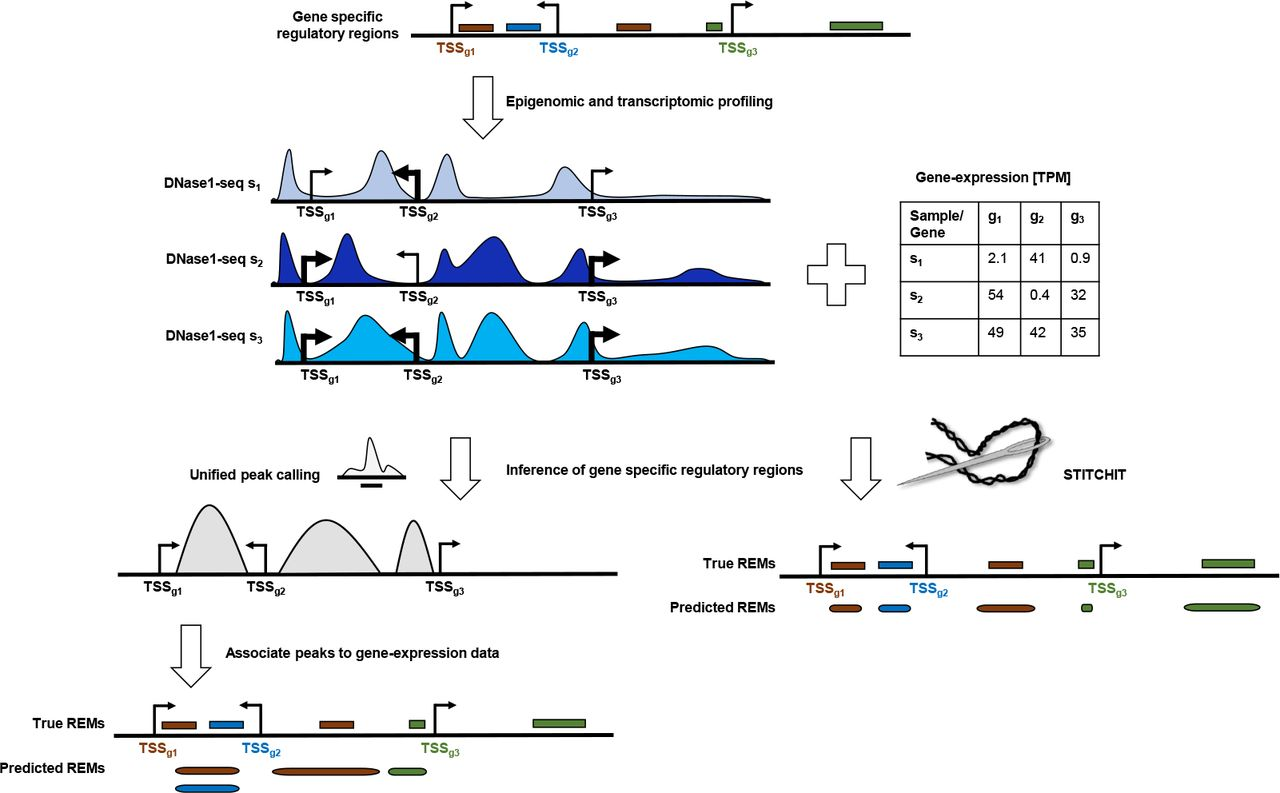
\includegraphics[scale=1.3]{figures/stitchit.jpg}}
	\caption{A Illustration of the STITCHIT method and its performance compared to peak-calling methods from the STITCHIT paper\cite{stitchit}.}
	\label{stitchit}
\end{center}
\end{figure}
REMs in EpiRegio are learned using STITCHIT\cite{stitchit}, which is a method to identify gene-specific REMs based on the analysis of epigenetic signal of diverse human cell types with respect to gene expression. STITCHIT does this by solving a classification problem in which it segments a large genomic area around the target gene(Fig. \ref{stitchit}). A linear regression using elastic-net penalty for feature selection and an Ordinary Least Squares regression to get a final regression coefficient and P-value are used. Regions exhibiting the epigenetic signal variance, which is linked to the expression of the gene, are highlighted in the resulting segmentation. Because STITCHIT is a peak-calling free approach it is able to identify REMs with high resolution and accuracy. Since genomic locations are not exclusive to REMs, REMs associated to different genes can overlap. Therefore Cluster of Regulatory EleMents (CREMs) are introduced, containing all, at least two, REMs overlapping with each other without any break in between. 
In EpiRegio mentioned REMs, CREMs and their target gene are stored with multiple attributes. REMs and CREMs are stored with unique IDs, chromosome, start position and end position. Genes are stored with their Ensemble ID, also chromosome, start position, end position and their expression value in the respective cell type and sample. The linkage between CREMs and REMs and genes has the following activity values. 

I) The \texttt{Model score} is a indicator on how important a REM is for the target gene expression compared to all other REMs assicated with that gene. The score is the absolute binary logarithm of the p-value of the regression coefficient for the connection between a REM and its associated gene. It is normalized with the maximal value to obtain a model score in the range [0, 1]. The larger the score, the more impact the REM has on the gene and vice versa. It is not cell type specific, thus can be used for comparison between REMs but not in between cell types.

II) The \texttt{StandDnase1Log2} score is a measurement for the accessibility of the chromatin in the REMs, indicating the activity of a REM to its target gene. It is the Deoxyribonuclease 1 (DNase1) signal for a REM retrieved from the Roadmap\cite{roadmap} and Blueprint\cite{blueprint} datasets. DNase1 is an endonuclease coded by the human DNASE1 gene, which functions by cleaving DNA in an endonucleolytic manner\cite{dnase_nih}. The signal is retrieved by the DNase 1-seq method\cite{dnase_method} and has been used as indicator for regulatory regions, which have been shown to map many types of cis regulatory elements. The DNase1 signal is log-transformed and standardized over all cell types\cite{dnase_cis}. The value inticates how active a REM is in a cell type for a sample and therefore allows the for the comparison between samples, since it is normalized for sequencing depth. 
\section{Gene regulation}
Gene regulation is a fundamental biological process necessary for the proper functioning of cells and organisms. Genes contain the instructions for making proteins, which perform essential tasks within cells, such as providing structural support, acting as transporters or catalyzing chemical reactions. However, not all genes should be active all the time. Gene regulation ensures that genes are activated or suppressed as needed to adapt to changing conditions and maintain cellular order. Therefore the regulation process is not static, they exhibit dynamic behaviors, responding to developmental cues and environmental stimuli\cite{GRN2}. 
\begin{wrapfigure}{r}{0.5\textwidth}
	\fbox{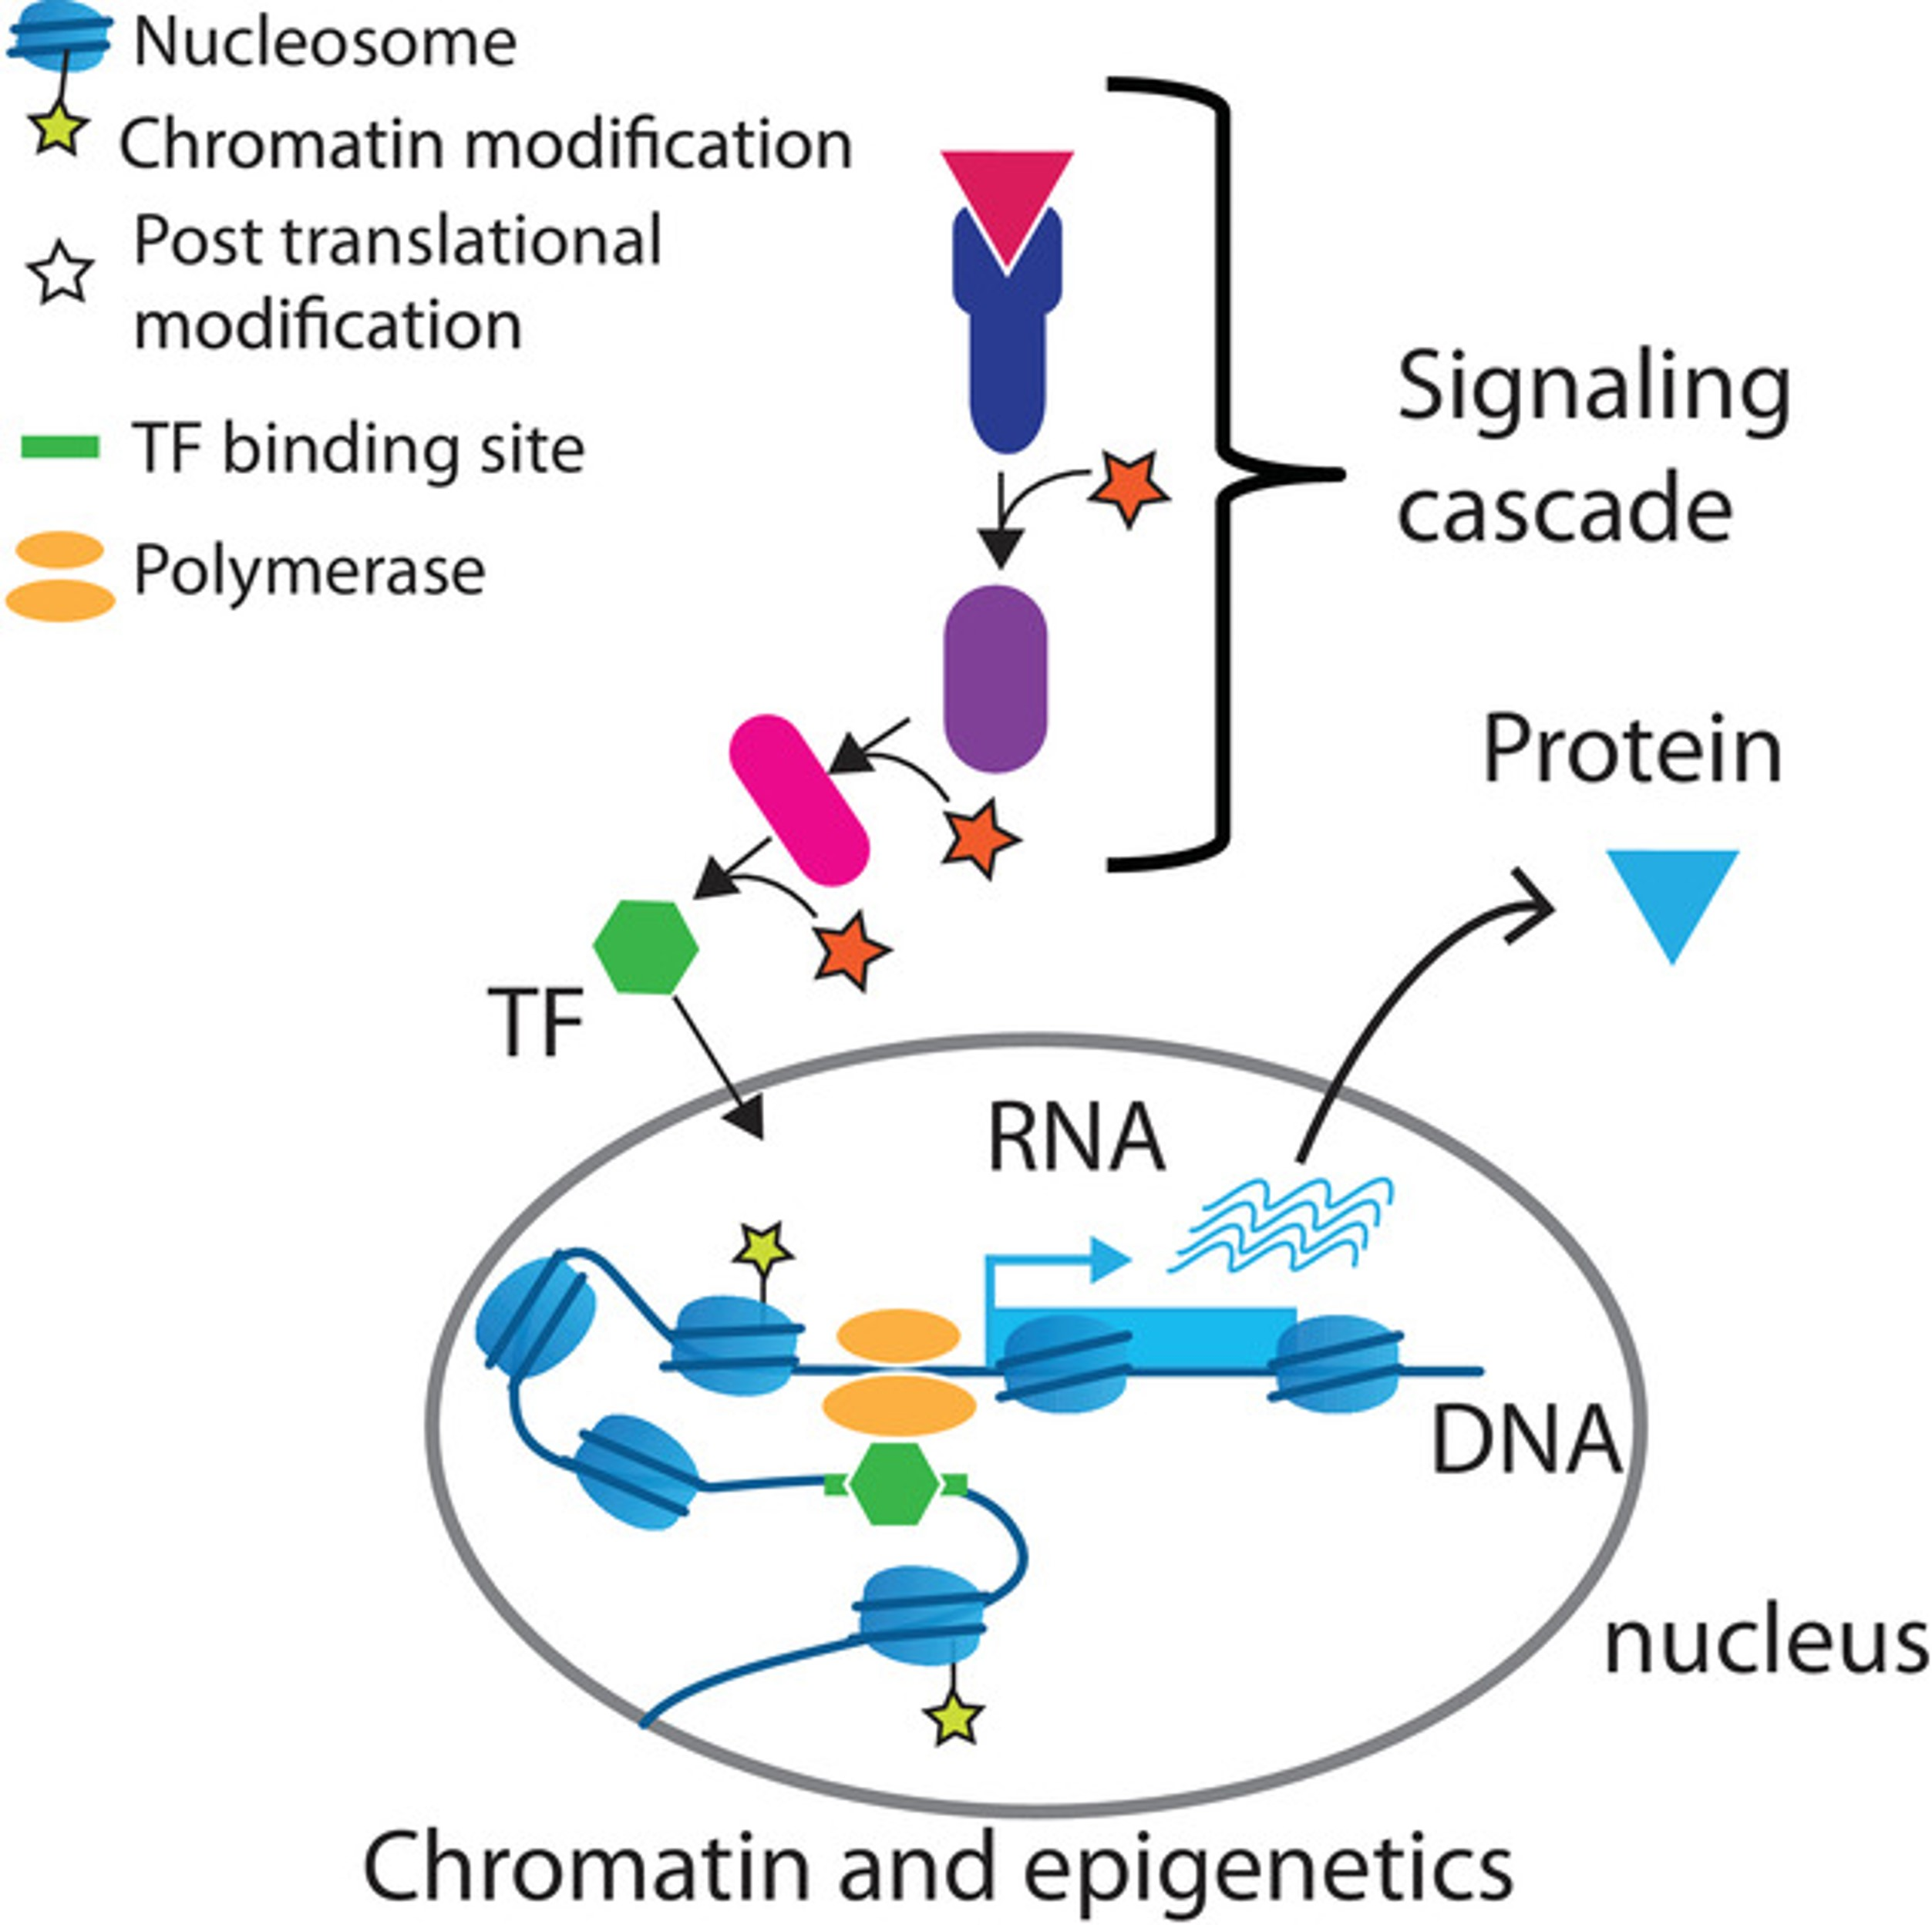
\includegraphics[scale=0.7]{figures/TF_function.jpg}}
	\caption{A simplified view of the TF activity in gene expression regulation\cite{TF_fig}.}
	\label{TF_function}
\end{wrapfigure}
This leads to a precise control over when and how much of a protein is produced, which crucial for the normal functioning of cells and the overall development of an organism.\cite{proteinfunction}.
Gene regulation relies on a complex system involving TFs, enhancers, and epigenetic modifications and often build a larger regulatory network. In this system TFs bind to specific DNA sequences in gene promoters and enhancers. By binding, they modulate the initiation and level of transcription, either activating or repressing gene expression. Activators facilitate the recruitment of RNA polymerase, essential for transcribing the gene into mRNA, while repressors inhibit this process (Fig \ref{TF_function}. These factors often operate in combinations, enabling precise and context-dependent control of gene activity. Epigenetic modifications, like DNA methylation and histone modifications, further modulate gene accessibility\cite{TFs}.

\subsection{Gene Regulatory Network}
Gene Regulatory Networks (GRNs) computationally model the mentioned regulation system of gene expression in living organisms\cite{GRN2}. 	

In GRNs the key players, TFs and genes, are represented as nodes connected through edges (Fig. \ref{network_webapp}). Edges contain a value describing the type and in what manner the TF regulates the genes expression. The edge weights can be either experimental, as already mentioned DNase 1 signals, or statistical values. Values from individual cell types can be used to create cell type specific GRNs to investigate in cell type specific regulations. 
The topology of GRNs varies, including hierarchical, modular, and feedback-driven structures. As gene regulatory systems are very complex, GRNs can become large and complicated. With centrality, clustering and other algorithms designed for large GRNs, these regulatory systems can be analyzed efficiently. The results are hoped to provide information about the pathways, structure and regulatory relationships between actors of the network\cite{GRN3}. 

Computational models and bioinformatics tools are essential for deciphering the complex dynamics of GRNs. 

\section{Dysregulation of DNA methylation in cancer}
Dysregulation of DNA methylation, the abnormal or altered methylation, is associated with various diseases, including cancer. Aberrant hypermethylation, the excessive methylation, of tumor suppressor gene promoter results in an inactivation of the gene. It contributes to oncogenesis and uncontrolled cell growth. On the other hand global hypomethylation, the reduced or absent DNA methylation, can activate oncogenes, fostering genomic instability\cite{MethCancer}.

Therefore these alterations and dysregulations in GRNs and DNA methylation are considered promising in cancer research and efforts are being made to find hypermethylated promoters as biomarkers for cancer. Understanding the mechanisms underlying the dysregulated systems is crucial epigenetic-based interventions in cancer treatment. Since DNA methylation is additionally reversible, it makes it vastly interesting in therapy research and is investigated in this work\cite{MethRole}.


\chapter{Methods}
\section{Packages}
The web application and all further analyses were created with the help of several libraries and all in Python and Jupyter Notebook. The fundamental ones include both dash\cite{dash} and graph-tool\cite{graph-tool}.

\subsection{Dash}
\label{dash}
Dash is an open source Python framework that can be used to efficiently create analytical web apps. Dash was used in this work to create the web app as a user interface for user interaction with the graphs. Therefore dash callbacks were used to integrate interactive elements such as filters, selections and file uploads. Dash and dash-bootstrap-components were used for drop-down menus, checklists, sliders, text inputs and buttons. For the graph display and interactive usage dash-cytoscape was used\cite{dash}.


\subsection{Graph-tool}
\label{graphtool}
Graph-tool is a python module that can be used to create, adapt, filter and analyse large networks. Since the library is implemented in C++, it has enormous advantages over other Python libraries. In terms of memory usage and computation time, it is comparable to a normal C++ library, which is significantly faster than a normal Python library. In graph-tool, graphs with their contained nodes, edges and corresponding attributes can be saved and reloaded in .gt-files (graph files). The gt file format provides a simple binary format as an alternative to the text based graphml format for large graphs. Where graphml files can be time and memory consuming for input and output for large graphs, the gt format handles these tasks in a compact and fast manner. In addition, many algorithms and other analysis tools are already integrated in the library\cite{graph-tool}.  

This makes it a perfect tool for the analysis of large regulatory networks and was used to integrate the graphs in this work. The graph files are integrated in the dash web app and can be reloaded when selected. They serve as base for the visualization with dash-cytoscape and can be filtered quickly.


\subsection{DysRegNet}

DysRegNet\cite{dysregnet} is a python package to detect patient-specific dysregulations within gene expression profiles. 
As input it requires a meta data table containing the meta data for all available samples, a GRN and an expression table containing the expression values for all nodes contained in the GRN. Additionally a number of filters and specified inputs can be given. 
As a result, it returns a table with a z-score for all edges contained in the GRN for each sample. The z-score indicates whether the edge in the disease sample is dysregulated compared to control samples and if so, how strongly. Positive values indicate activation and negative values indicate repression, the value 0 indicates that this edge is not significantly dysregulated. 
\begin{figure}[!ht]
\begin{center}
	\fbox{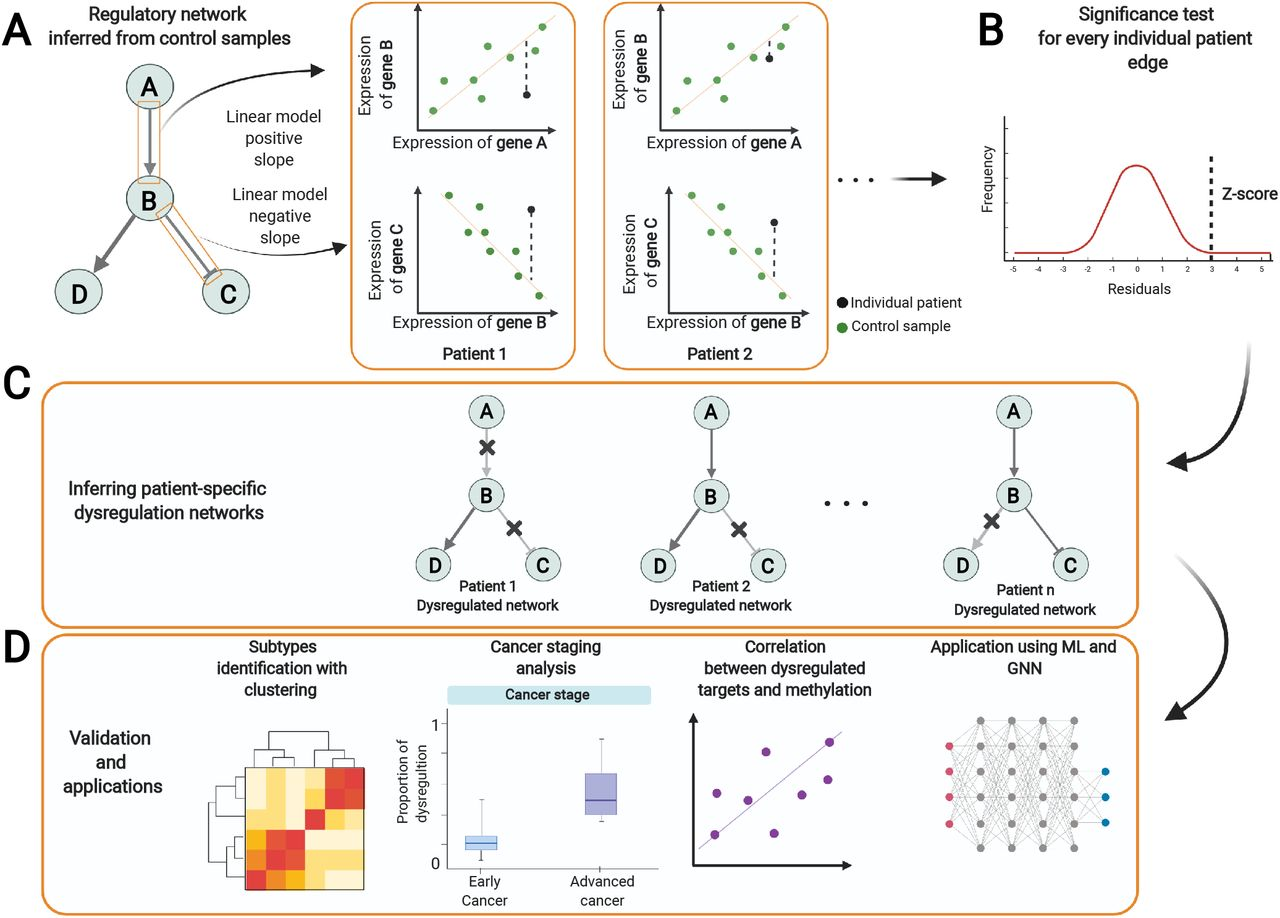
\includegraphics[scale=1.3]{figures/dysregnet.jpg}}
	\caption{A Illustration of the DysRegNet tool and workflow. Showing the fitting of the linear model for each edge, the patient individual significance test, the resulting networks and the subsequent result validation\cite{dysregnet}.}
	\label{dysregnet}
\end{center}
\end{figure}

DysRegNet does this by fitting a linear model for each edge using all control samples given by the input GRN. Then each patient sample is tested one after the other and the observed value is compared with the expected value from the linear model and transformed to a z-score. The results can then be validated using known data. 


\section{Network generation and data preparation}
\subsection{Graph-files}
\label{graphfiles}
For the creation of the graph files, all 10 files of the EpiRegioDB were viewed and all samples from the \texttt{sampleInfo\_Roadmap\_1.csv} and \texttt{sampleInfo\_Blueprint\_1.csv} project files were assigned to their cell types with help of the \texttt{CellTypeInfo.csv} file. The samples from both projects were matched with those of the \texttt{REMActivity\_1.csv} file. This resulted in 165 samples in 46 cell types which are stored in the \texttt{sampleToCelltype.csv} file. 

For each cell type, a directed graph file was created containing the edge, the REM and the gene as source and target node from the \texttt{REMAnnotationModelScore\_1.csv} file. As an edge attribute the cell type specific edge weights contained in the cell type were stored as an internal \texttt{edge\_property} from graph-tool under the sample name. As edge weight the value of the standDnase1Log2 column from the \texttt{REMActivity\_1.csv} file was used. REMs associated with a CREM from the \texttt{clusterREMs\_1.csv} file were merged into one CREM node. CREMs have a single edge to the corresponding gene for each contained REM. 

In addition, a graph file with the identical edges, genes and REMs as nodes was created using the \texttt{REMAnnotationModelScore\_1.csv} file. As edge weight the value of the normModelScore column from the same file was used, which contains the model score across all cell types.
As REM and gene internal \texttt{vertex\_property} node attributes, type, name, chromosome, start, end and for the cell type specific graph files the gene expression for gene nodes for the respective sample were added from \texttt{GeneExpressionBlueprint\_1.csv} and \texttt{GeneExpressionBlueprint\_1.csv}.
As additional edge attributes the rem name of the edge, for the model score graph file the p-value and for the cell type specific graph files the cell type and cell type ID were added. 

As already mentioned, depending on whether it is a cell type specific or the model score graph, the edge and node attributes differ. To show the attributes values an example the graph for \texttt{CTID\_0000006}, cd14-positive monocyte and the model score graph is taken. 
\paragraph{Node attributes:} 
\begin{itemize}
\item name: name of the gene/REM
\item type: node type, either gene oder rem
\item chr: chromosome on which the gene/REM in located
\item start: start coordinate of gene/REM
\item end: end coordinate of gene/REM
\end{itemize}
Only for gene nodes:
\begin{itemize}
\item B\_C0010KB1: expression value in sample B\_C0010KB1
\item B\_C0011IB1: expression value in sample B\_C0011IB1
\item B\_C001UYB4: expression value in sample B\_C001UYB4
\end{itemize}
The model score graph has all these node attributes except for the expression values. The reason for this is that this graph contains model score values for all cell types and therefore has no expression value for all cell types at once. 
The difference with the CTID\_0000006 graph concerning the edge attributes is that it has a separate edge attribute for each sample with its name. 
\paragraph{Edge attributes:} 
\begin{itemize}
\item rem: REM name the edge is assigned to, only important if REM is part of a CREM
\item celltype: CTID\_0000006
\item celltypeID: cd14-positive monocyte
\item B\_C0010KB1: standDnase1Log2 value for edge in sample B\_C0010KB1
\item B\_C0011IB1: standDnase1Log2 value for edge in sample B\_C0011IB1
\item B\_C001UYB4: standDnase1Log2 value for edge in sample B\_C001UYB4
\end{itemize}
In the model score graph, the same attributes are present except for the standDnase1Log2 values, these are replaced by the following:
\begin{itemize}
\item score: model score over all cell types
\item p-value: p-value for the model score
\end{itemize}
This gives us 47 graph files in total with identical nodes and edges, each representing a cell type specific or general GRN.

\subsection{CpG-mapping and beta-values}
To use the GRN as input to DysRegNet an expression value for each node is needed. So far, the GRNs only contain expression values for gene nodes. To obtain expression values for the REMs as well, the beta-values of all CpGs lying within the REM coordinates from Illumina Methylation450K\cite{methylation450} were used. 

Since the coordinates of the CpGs are based on GRCh37 and all EpiRegio coordinates are based on GRCh38, the CpG coordinates were mapped to GRCh38 using UCSC LiftOver with default settings\cite{liftover}. LiftOver takes a bed file containing the input coordinates from the selected assembly and convertes them to the coordinates of the desired output assembly. Coordinates that can't be converted result in a list of mismatches, the successfully converted coordinates are printed to a file. After manually filtering 71 mismatches from LiftOver and REMs to which no CpG site could be assigned, all remaining REMs have their assigned CpGs by mapping the CpG site coordinates to the REM coordinate ranges.

The beta-values of the CpGs were converted to m-values, as these show significantly better performance in identifying differentially methylated CpG sites\cite{mvalues} by the following equation:
\begin{equation}
	m-value = \log_{2}{(\frac{beta}{1-beta})}
\end{equation}
To obtain a single expression value for a REM, the mean was calculated over all m-values of the CpGs contained in a REM.

This provides all input data, the GRN, expression values for all nodes, and the remaining data of respective dataset for DysRegNet.

\chapter{Results}
\section{Network}
The resulting 47 gene regulatory networks serve as the basis for all analyses and visualizations. These very large networks contain several million nodes and edges. In detail every graph consists of:

\renewcommand{\arraystretch}{2}
\begin{table}[!ht]
\centering
\begin{tabular}{|c|c|}
\hline
Number of nodes		& 1.541.001		\\
Number of edges		& 2.404.861		\\
Number of genes		& 35.379        \\
Number of REMs		& 1.140.336		\\
Number of CREMs		& 365.286      	\\
\hline
\end{tabular}
\caption{Element numbers contained in the network graph.}
\label{numbers}
\end{table}
\renewcommand{\arraystretch}{1}
The basic structure of the graphs is composed of small clusters consisting of one gene, which has a large number of incoming edges from REMs and CREMs (Fig. \ref{network}). Genes have exclusively named incoming edges and no edges to other genes. REMs have exclusively a single outgoing edge to their assigned gene and no edge to other REMs. Only CREMs have multiple outgoing edges representing the edges of the contained REMs. CREMs can therefore also have edges to several different genes or several edges to the same gene, each representing a single REM edge. Thus, the mentioned small clusters are connected, if then only by edges from CREMs. Since not every gene has an edge to a CREM and only through it can the individual gene clusters be connected, the network is a disjoint network.
 
Fig. \ref{network_webapp}, a section of the webapp visualization, illustrates the individual cases all at once. Three genes can be seen as light blue nodes, REMs and CREMs are shown as black nodes and are all connected by their edges. \texttt{ENSG00000142627} in the upper right corner shows the case where a gene is connected only to REMs and not CREMs, creating an isolated clique with no connection to the rest of the network because REMs can exclusively have a single edge to a gene. The large cluster in the lower left center of the figure with \texttt{ENSG00000236908} and \texttt{ENSG00000275850} shows how two genes are connected via \texttt{CREM0068412}. Here, \texttt{ENSG00000236908} has only one incoming edge through the mentioned CREM and \texttt{ENSG00000275850} forms a cluster with several neighboring REMs and CREMs, while it is also connected to other genes via the latter, but these are not shown here. Also, one can see the case where a CREM has multiple edges to the same gene, each representing a separate REM edge.
\begin{figure}[!ht]
\begin{center}
	\fbox{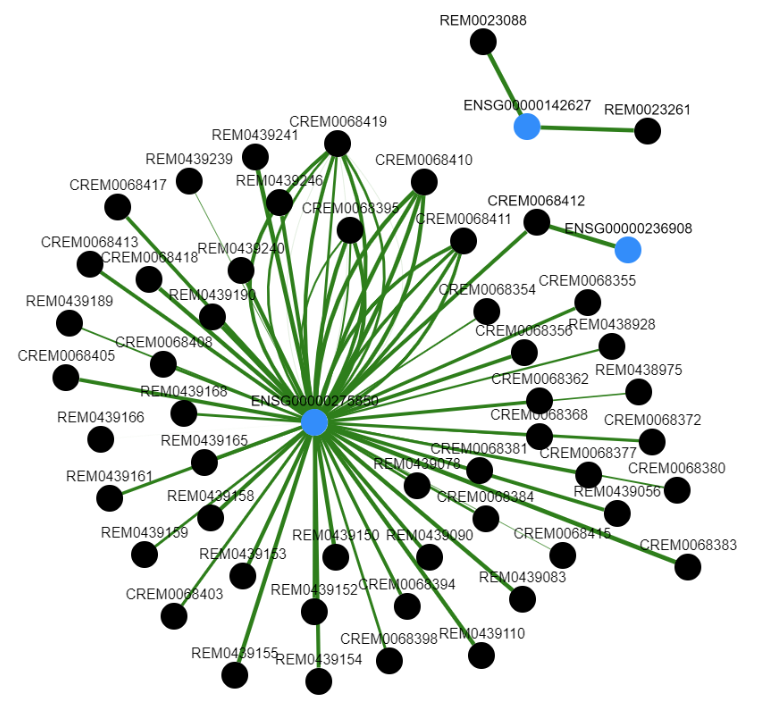
\includegraphics[scale=0.597]{figures/network_webapp1.png}}
	\caption{Visualization of three genes and their connected REMs and CREMs in the Webapp showing the clusters and disjoint structure of the network.}
	\label{network_webapp}
\end{center}
\end{figure}

Looking at the topology, the graph consists of 2,188 individual components, which are shielded from each other and cannot be reached by each other. The sizes of the components range from 2 to the largest component with 16,500 contained nodes and form a total of 1055 different sizes. Smaller components with up to 1,000 contained nodes occur significantly more often than extremely large ones. The most frequent components are those with 55 nodes, of which a total of 134 can be found in the entire network, and the least frequent components with 10,000 nodes or more are usually represented only once. That illustrates that the network consists of many individual components, which differ strongly by their size and frequency.
\begin{figure}[!ht]
\begin{center}
	\fbox{
\includegraphics[scale=0.597]{figures/REMnet2.JPG}}
	\caption{Part of the model score network graph visualized with Cosmograph\cite{cosmograph} showing the clusters with one gene and multiple REMs and CREMs}
	\label{network}
\end{center}
\end{figure}

The average degree over all nodes within the graph is 3.12, but it differs enormously if you look at the type of nodes. The average degree for gene nodes is 67.97 and for REM and CREM nodes only 1.60. This value is so low for REM and CREM nodes, because REMs always have only one edge to a certain gene and thus drive the average value strongly down. Looking at the average degree for CREMs only, it is almost three times higher at 3.46. These numbers again describe the network structure with clusters of genes with many edges to regulatory elements. The value of the maximum degree does not differ that much and is 108 for gene nodes and 122 for CREMs, for REMs the value is self-explanatory 1.0. However, 8096 genes have a degree of 108, but only \texttt{CREM0109128} has a degree of 122. 
The degree distribution of the CREMs (Fig. \ref{crem_degree}) is very one-sided and most of them have degrees of 2 and from fifteen on there are only a few with higher degrees. The distribution of gene degrees (Fig. \ref{gene_degree}), on the other hand, looks very different with two maxima at 54 and 108, showing us that a maximum degree of 108 is a common case. 

Results that support these findings can also be seen by looking at the clustering coefficients, which give 0 for both local and global clustering coefficients.  For this purpose the methods \texttt{local\_clustering} and \texttt{global\_clustering integrated} with default settings from graph-tool were used. These minimal coefficients tell us that all nodes in this network have no edges between their neighboring nodes, and thus only nodes are connected to their immediate neighbors. This confirms the description of the basic network structure as described earlier.

CENTRALITY???

How to check which TF in CREM0109128 location ???






\section{Web application}
To be able to interact with the created graph files, a user friendly web application (app) was designed. The app offer to visualize, interact and filter the networks and their properties for user specific usage. It was created as described in \ref{dash} using dash and dash-cytoscape.
%The following is the structure and a description of the functions and filters of the app. 

\subsection{Structure}
The basic structure of the app is divided into three parts, which are arranged vertically next to each other. In the left column, the data can be selected for display and there is the option for a file upload. In the middle column is the display area of the elements selected in the left column. In the right column you can filter the elements to be visualized and display information about selected nodes. 

\begin{figure}[!ht]
\begin{center}
	\fbox{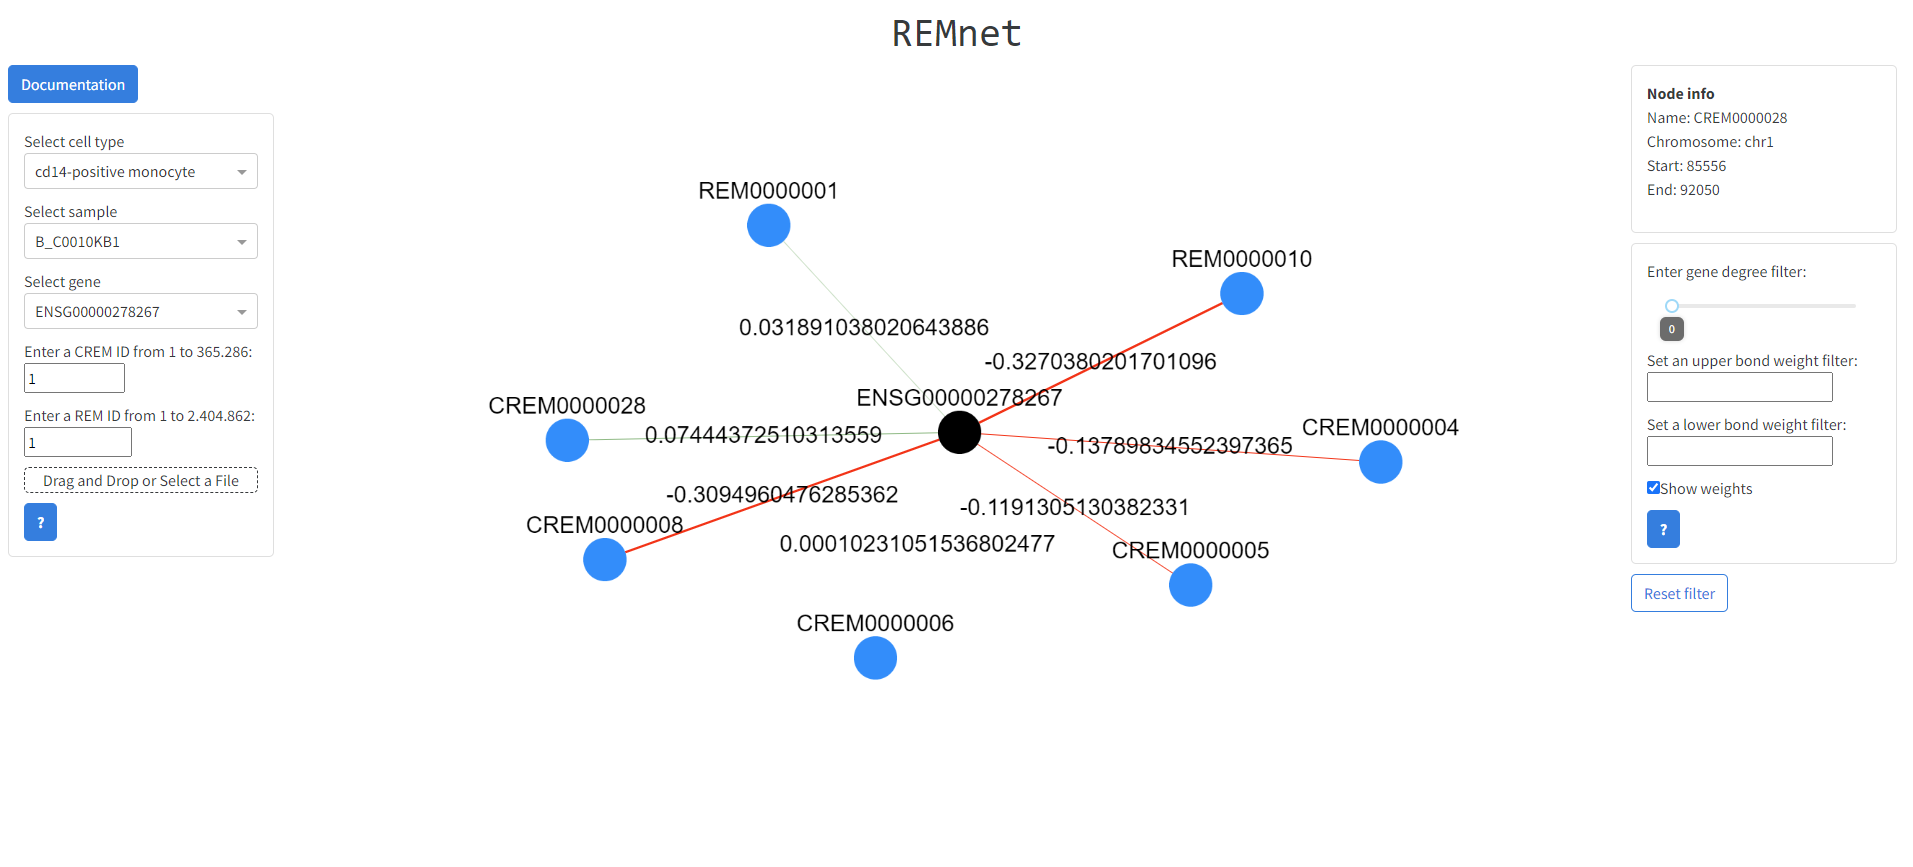
\includegraphics[scale=0.389]{figures/webapp.png}}
	\caption{App view on start with the selection options on the left, the visualization in the middle and the filtering on the right.}
	\label{webapp}
\end{center}
\end{figure}

The left column is the selection column. It has two help buttons for the user, right at the beginning with the Documentation button, which gives an overview of which actions can be performed in which parts of the app. This window can be opened and closed like the other two \texttt{?} help windows by simple clicks. 

Below that is the window for all display choices. In the first \texttt{Select cell type} drop-down menu, you can choose from all cell types contained in Roadmap\cite{roadmap} and Blueprint\cite{blueprint}. Selecting one of the cell types will reload the respective graph file as described in \ref{graphtool}. This results in a short loading time, but it allows to speed up the subsequent work in the graph file. For the loading time a spinning loading circle is displayed in the upper center of the page. Below that, it is possible to choose from all the samples available for this cell type in the \texttt{Select sample} drop-down. If the graph for all cell types is selected, the model score and the p-value are selectable instead of the sample names as explained in \ref{graphfiles}. In the next three input fields, genes, REMs or CREMs can be selected. Only one of the three can be shown in the visualization, the last selection is always shown. In the gene \texttt{Select gene} drop-down menu, genes can be selected by their ensemble ID. For the selection of REMs and CREMs, the desired ID must be entered. All drop-down menus can be searched for the desired selections. 

In addition to the above options, the user can upload a CSV file with individualized nodes and edges. This function is useful if only selected or several disconnected elements are to be displayed. The file must be in the format \texttt{'REM,GENE'} as header with two columns where each row describes an edge between the respective REM and Gen. Other file formats and formattings are not accepted. The \texttt{?} help button gives instructions to the user on how to use the selection and upload options.

\subsection{Visualisation}
In the app center, individual genes, REMs, CREMs and their neighboring nodes and edges can be displayed or a user-defined input of nodes by the file upload.

When a gene, REM or CREM is selected, it is displayed as seed node in black. All neighboring nodes are displayed in light blue and the edges leading to them. Above each node the corresponding name is displayed. Depending on the previously selected sample, the adjusted edge weights are shown on the edges. For a simplified illustration, the edges are colored green for positive edge weights and red for negative edge weights. In addition, the edge width adapts to the weights and becomes wider the further away the value is from 0. If the file upload function is used, all edges specified in the file are displayed. Genes are always displayed as black nodes and REMs and CREMs as light blue nodes (Fig. \ref{network_webapp}). 

These display options were chosen because the display of the entire GRN is not useful for several reasons. On the one hand, it would be extremely inefficient, creating long loading times and thus a poor user experience. On the other hand, the display of the entire GRN would be confusing and the user would have difficulties to orientate himself, as in Fig. \ref{complete_network}. 

\subsection{Filtering}
The right column of the app contains information about nodes and filtering options for the GRN. 

In the upper bin, information about nodes for which more details are requested can be displayed. The information appears by simply clicking on a node. The name of the node, on which chromosome it is located and the start and end position in the genome are given. The display is available for genes as well as REMs and CREMs. 

The box below contains the filter options for the network visualization. With the help of the first \texttt{Enter gene degree filter} slider the gene degree can be filtered. By moving the slider, genes with a higher gene degree than the filter value are filtered. This affects the \texttt{Select gene} dropdown menu where the selectable genes are adjusted according to the filter. In the \texttt{Upper bond weight filter} and \texttt{Lower bond weight filter} input fields the edge weights can be filtered. In the former, edge weights smaller than the filter are filtered and larger ones are left out. With the latter it is the opposite, edge weights larger than the filter are filtered and smaller ones are left out. Thus, the edge weights can be narrowed down from both sides. The filters are transferred to the visualization after selection and all edges excluded by the filters and nodes connected only by the excluded edge are removed. Using the \texttt{Show weights} select box, the edge weights can be shown or hidden. The \texttt{?} help button gives instructions to the user on how to use filters correctly. The \texttt{Reset filter} button resets all selected filters to their default values. 

All these functions and filters together form the web app, which allows the user to view and filter desired parts of the GRN.  
\section{Use case}
\subsection{TCGA}
\subsection{DysRegNet}

\chapter{Discussion}
\begin{itemize}
	\item discuss results
	\item how to use web app
	\item how to interpret genes and rems
	\item select multiple genes
	\item select network components
	\item more filter, gene filter both directions
\end{itemize}


\medskip
\clearpage
\bibliographystyle{unsrt}
\addcontentsline{toc}{chapter}{References}
\bibliography{references}

\pagebreak
\appendix
\chapter{Appendix}
\section{Figures}
\begin{figure}[!ht]
\begin{center}
	\fbox{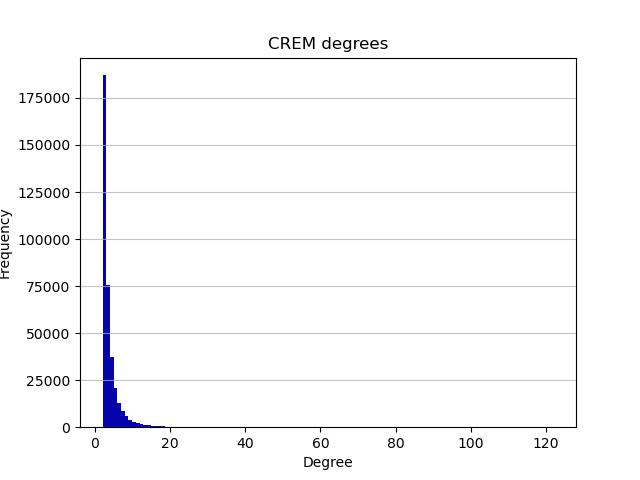
\includegraphics[scale=0.7]{figures/crem_degree.jpg}}
	\caption{Distribution of CREM degrees in GRN.}
	\label{crem_degree}
\end{center}
\end{figure}

\begin{figure}[!ht]
\begin{center}
	\fbox{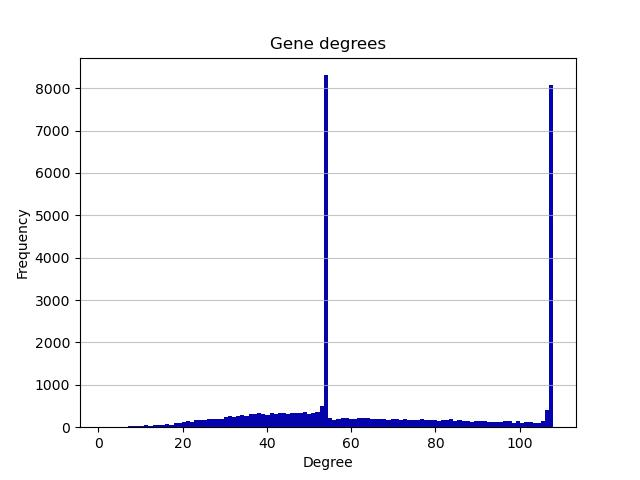
\includegraphics[scale=0.7]{figures/gene_degree.jpg}}
	\caption{Distribution of gene degrees in GRN.}
	\label{gene_degree}
\end{center}
\end{figure}

\begin{figure}[!ht]
\begin{center}
	\fbox{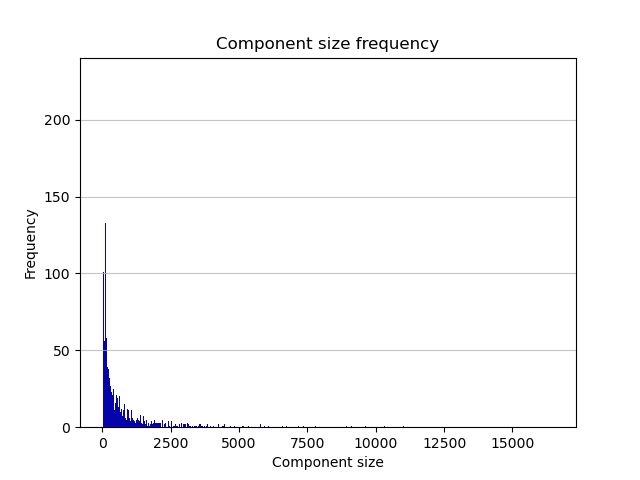
\includegraphics[scale=0.7]{figures/comp_size_freq.png}}
	\caption{Frequency of all component sizes in the network.}
	\label{comp_freq}
\end{center}
\end{figure}

\begin{figure}[!ht]
\begin{center}
	\fbox{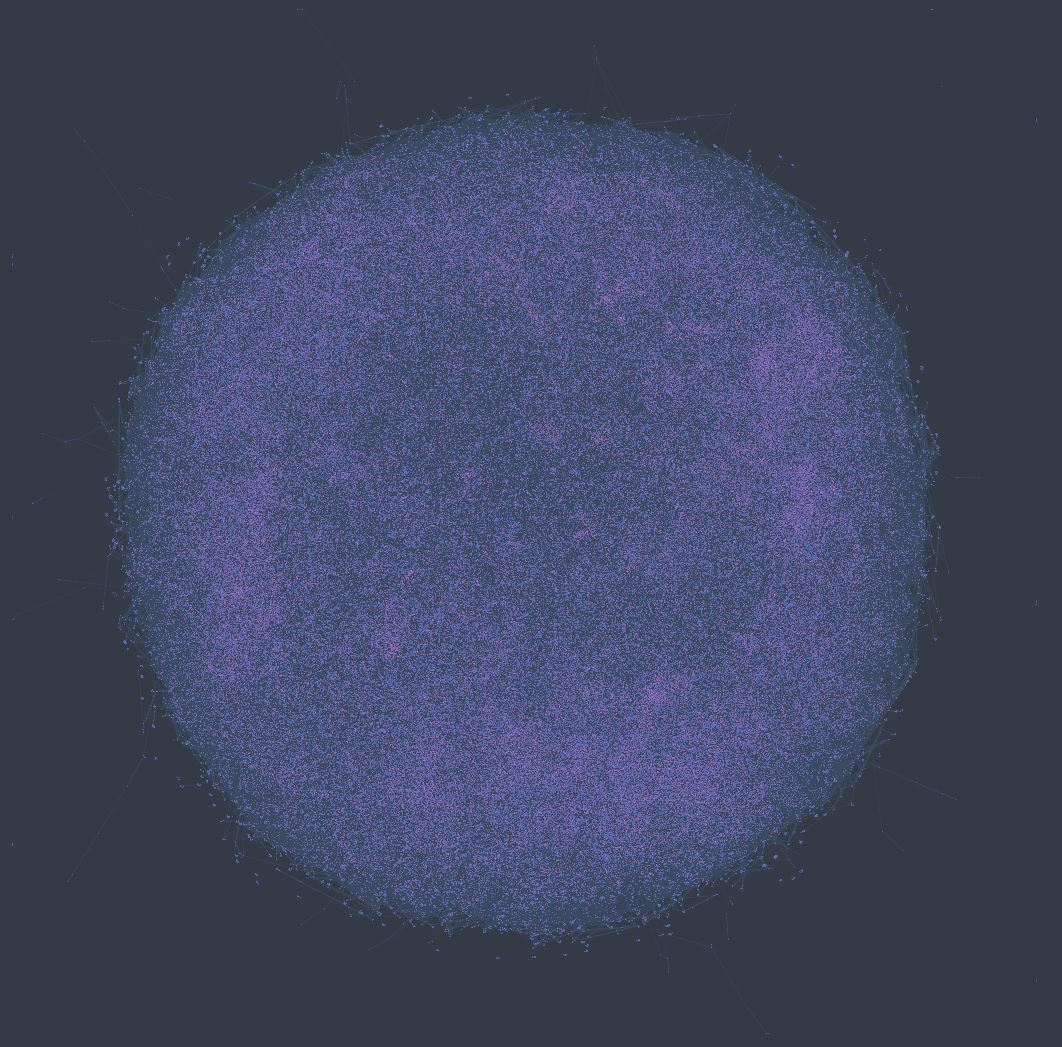
\includegraphics[scale=0.7]{figures/REMnet_rund.jpg}}
	\caption{Visualization of the entire with all nodes and edges with cosmograph\cite{cosmograph}.}
	\label{complete_network}
\end{center}
\end{figure}

\end{document}